\chapter{Experiments}
In this chapter, we are going to analyze the evolution and final results of the two models (see chapter \ref{methods:both_models}), trained on the OpenSubtitles and Reddit corpus, under several different aspects:

\begin{enumerate}[noitemsep]
	\item \textbf{Quantitive}: This part focuses on evaluating metrics and other measurements. We are going to look into the metrics at train time, a similarity analysis using Sent2Vec and an analysis of the produced language models by using n-gram collocations.\todo{Not correct: What are we going to do with ngrams?}
	\item \textbf{Qualitative}: This part focuses on the quality of the language produced by the models. This includes a comparison between our models and \emph{CleverBot}\footnote{http://www.cleverbot.com/} and the development of the language model of the models throughout the training time.
	\item \textbf{Miscellaneous}: This part focuses on theoretical analysis, such as analyzing the internal embeddings for the input sequence or if and how the models are using the soft-attention mechanism in their favor.
\end{enumerate}
\blindtext

* Attention
* Learning process
* Generated outputs over time
* Generation at the end and comparison with cleverbot and paper
* Generated outputs at the end and related ngram analysis
* Generated embeddings for input sentences
* Sent2Vec analysis


\section{Analysis of Learning Process}
\blindtext

\begin{figure}[H]
	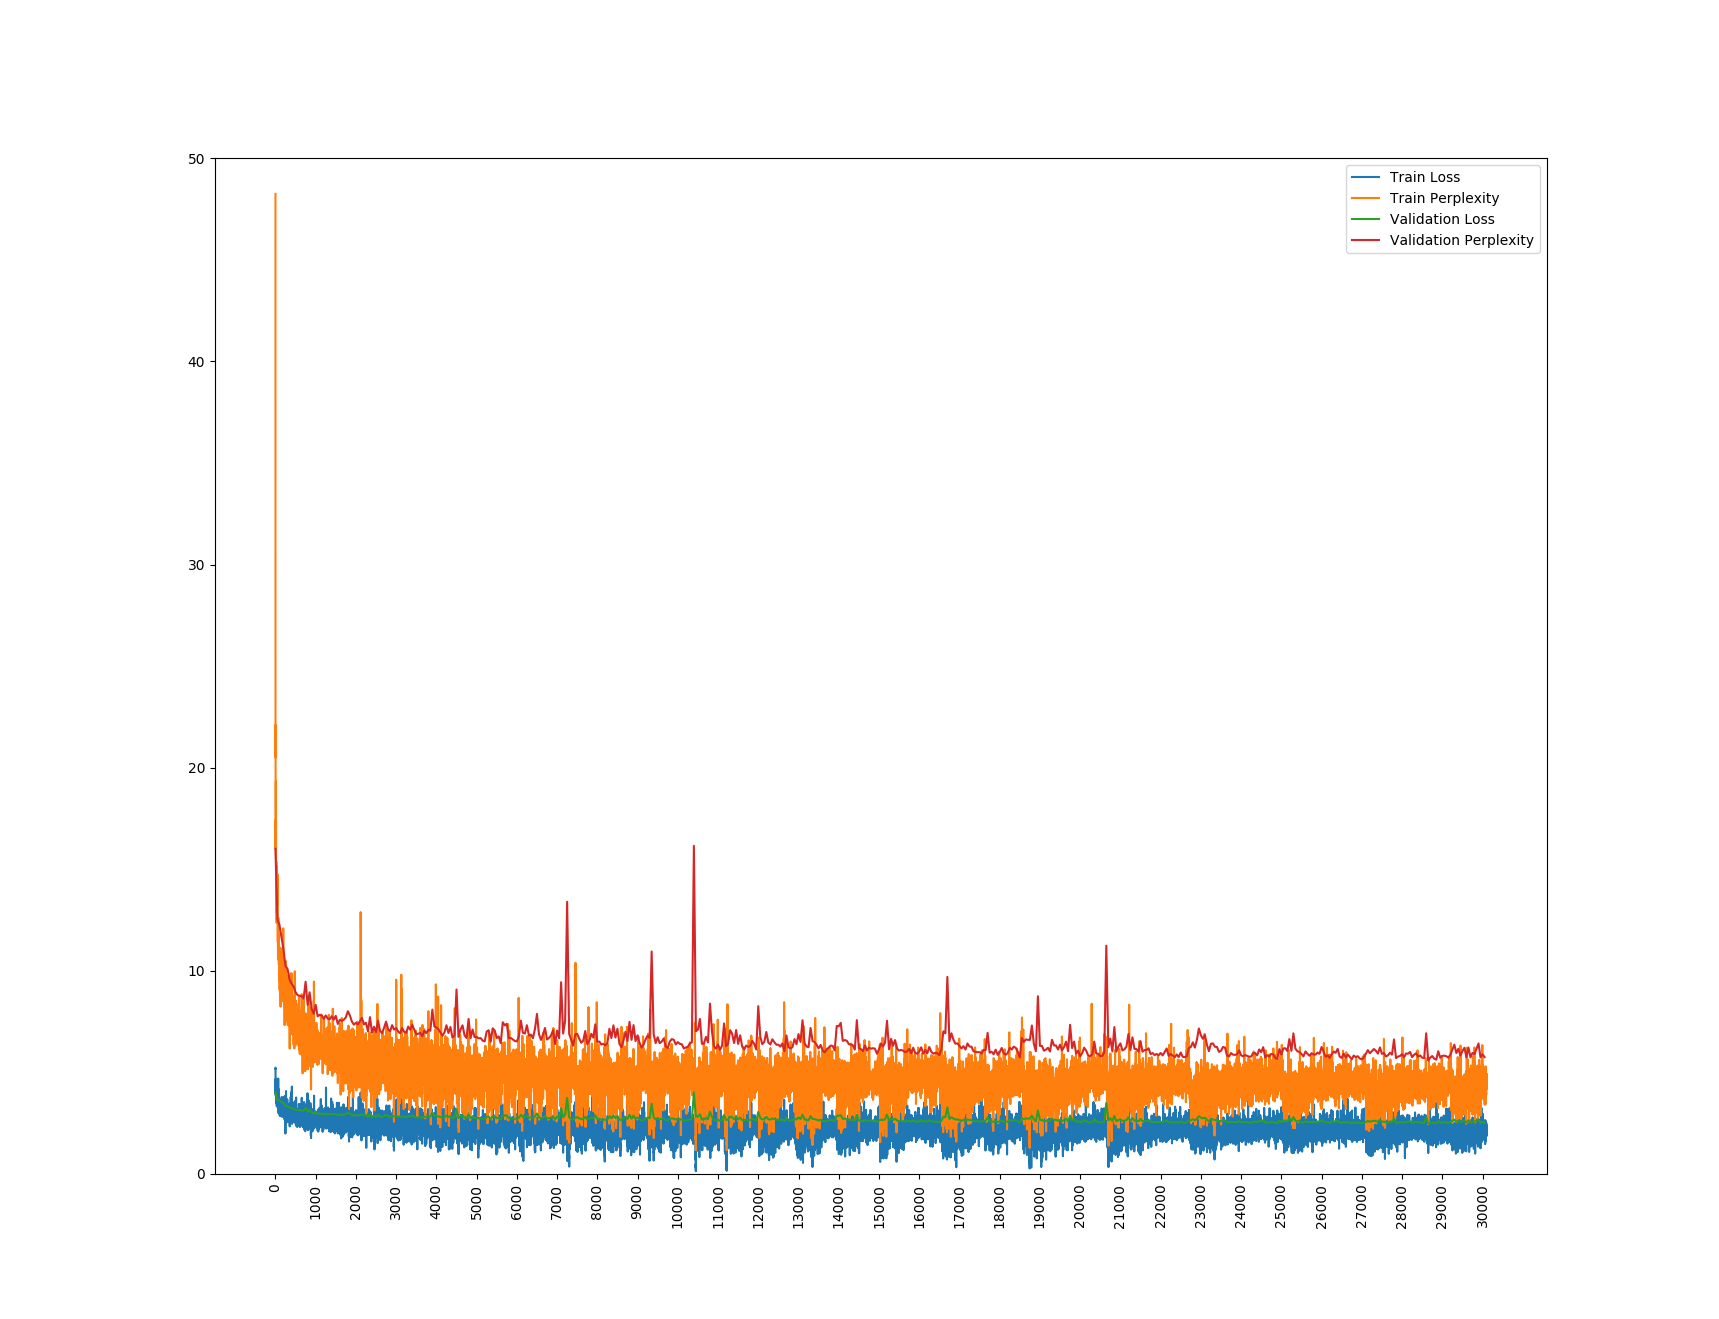
\includegraphics[width=\linewidth]{img/plots/opensubtitles_not_reversed/train_metrics.png}
	\caption{Development of the loss and perplexity on the training and validation set throughout the training of the OpenSubtitles model.}
	\label{results:learning_process:metrics:opensubtitles}
\end{figure}

\begin{figure}[H]
	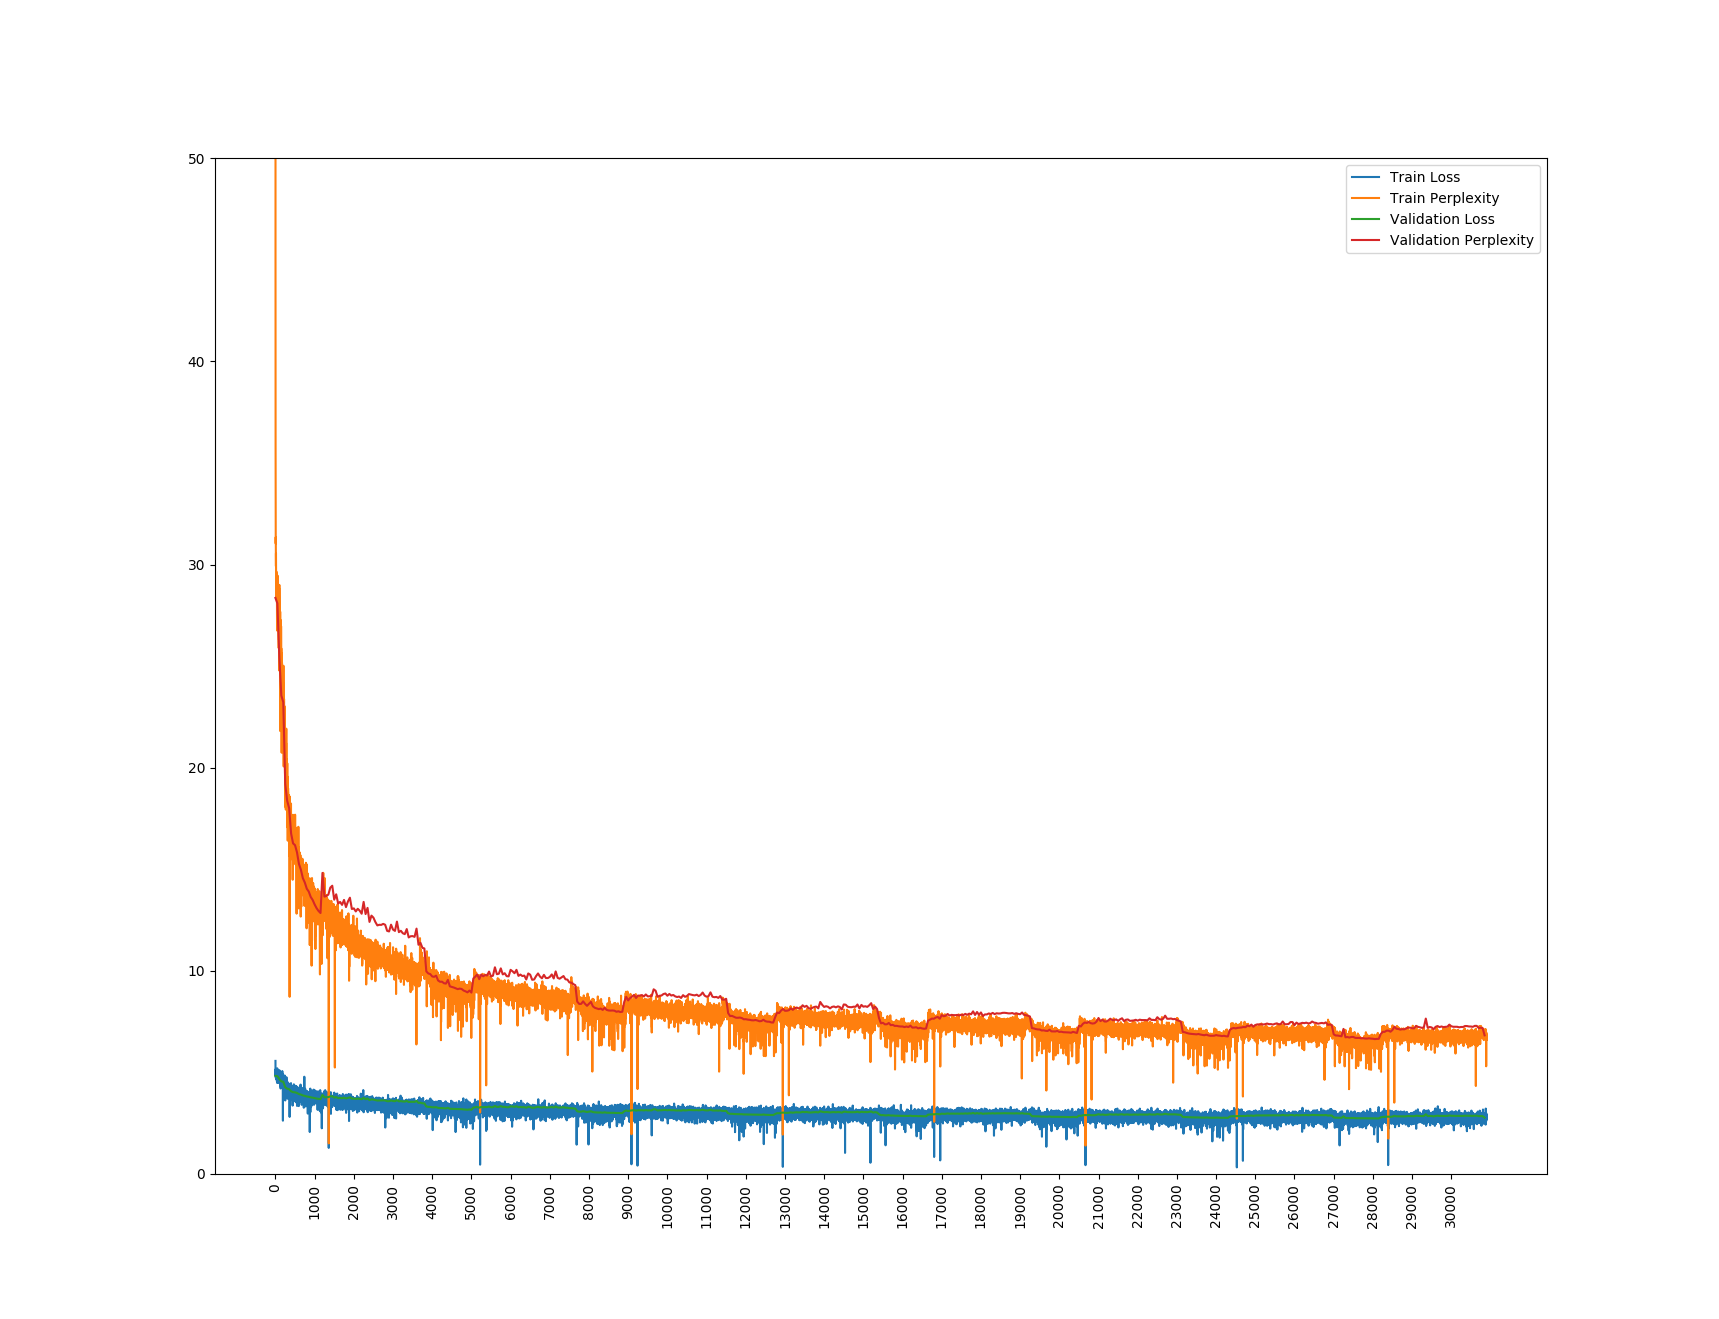
\includegraphics[width=\linewidth]{img/plots/reddit/train_metrics.png}
	\caption{Development of the loss and perplexity on the training and validation set throughout the training of the Reddit model.}
	\label{results:learning_process:metrics:reddit}
\end{figure}

\section{Performance on Test Sets}

\begin{figure}[H]
	\minipage{0.5\textwidth}
	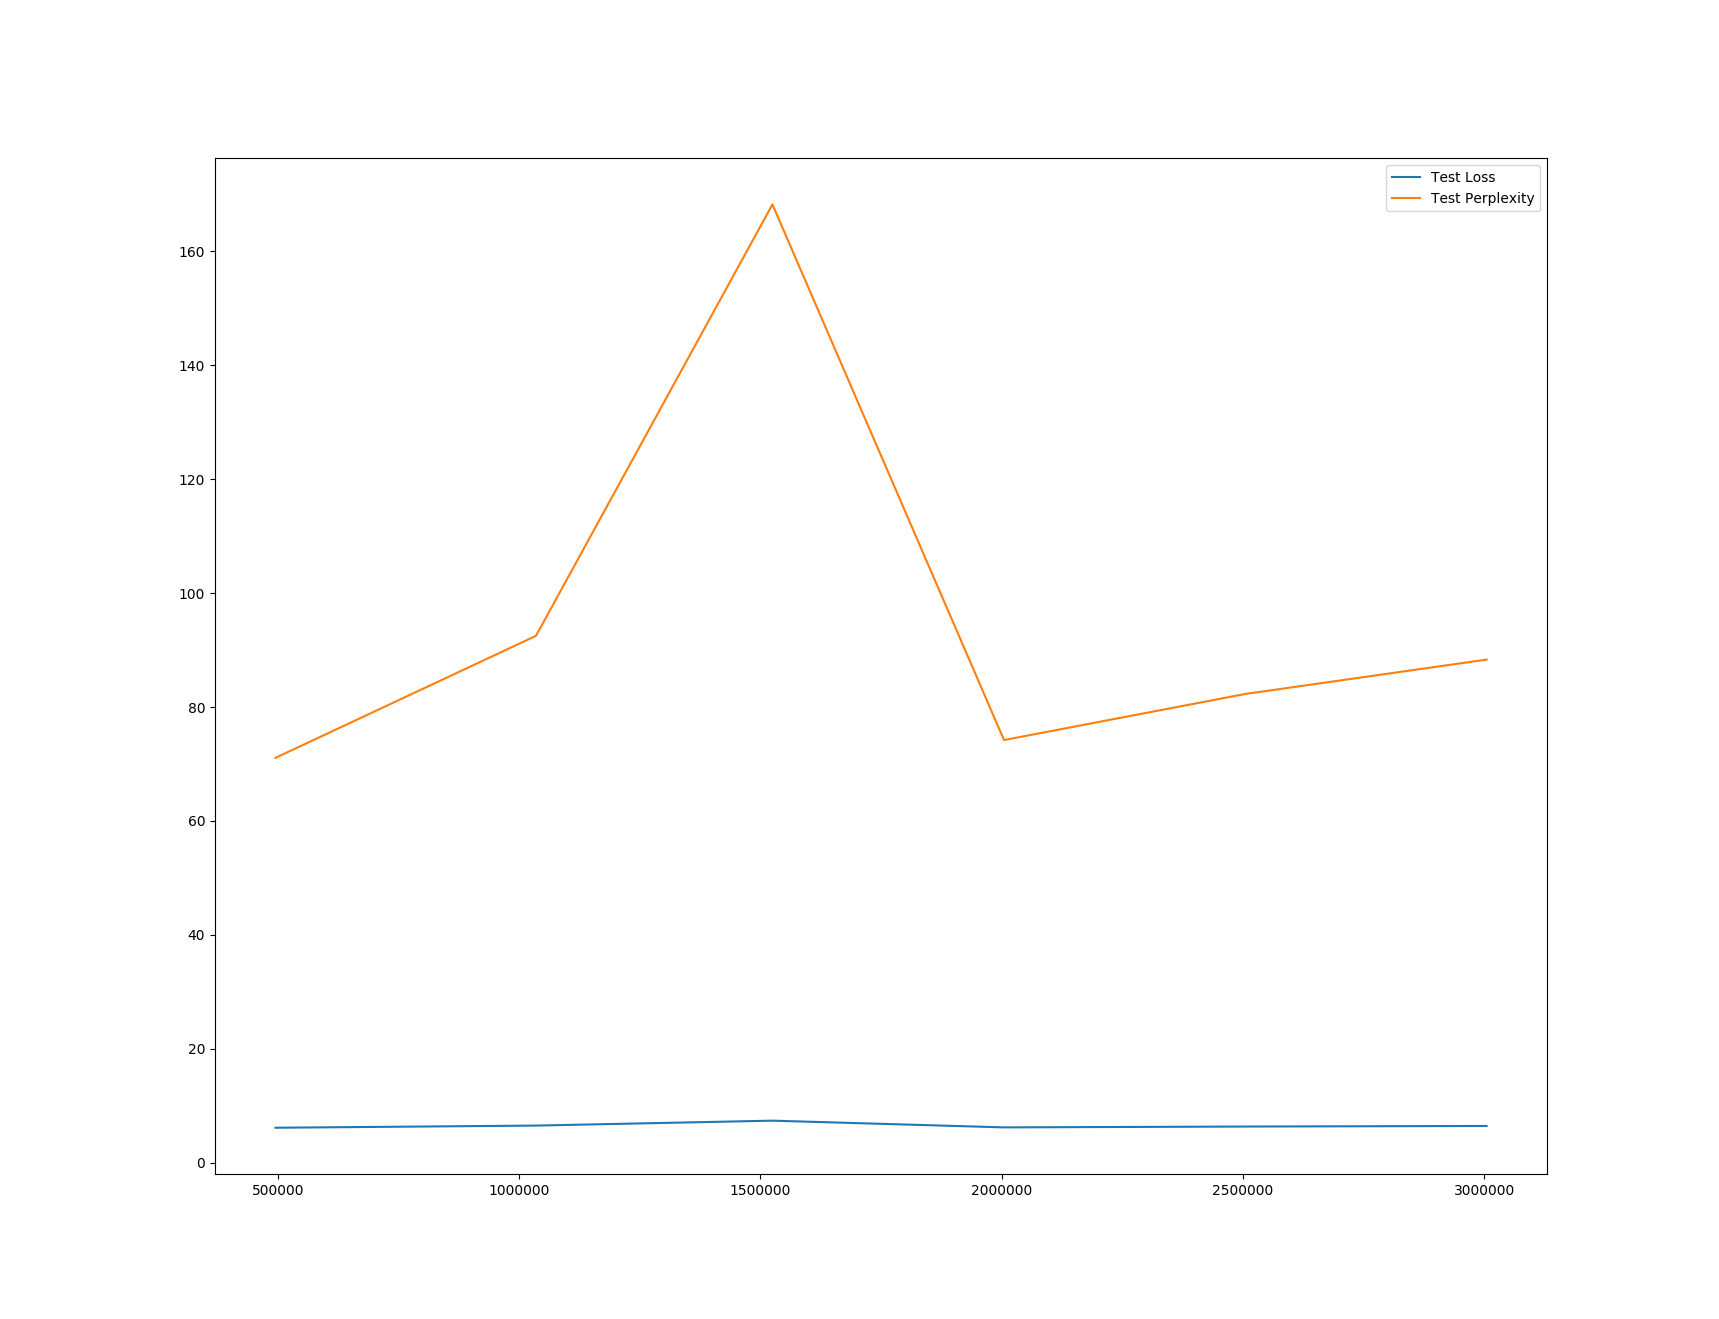
\includegraphics[width=\linewidth]{img/plots/opensubtitles_not_reversed/test_metrics_both.png}
	\centering
	\small
	\text{The loss and perplexity.}
	\endminipage\hfill
	\minipage{0.5\textwidth}
	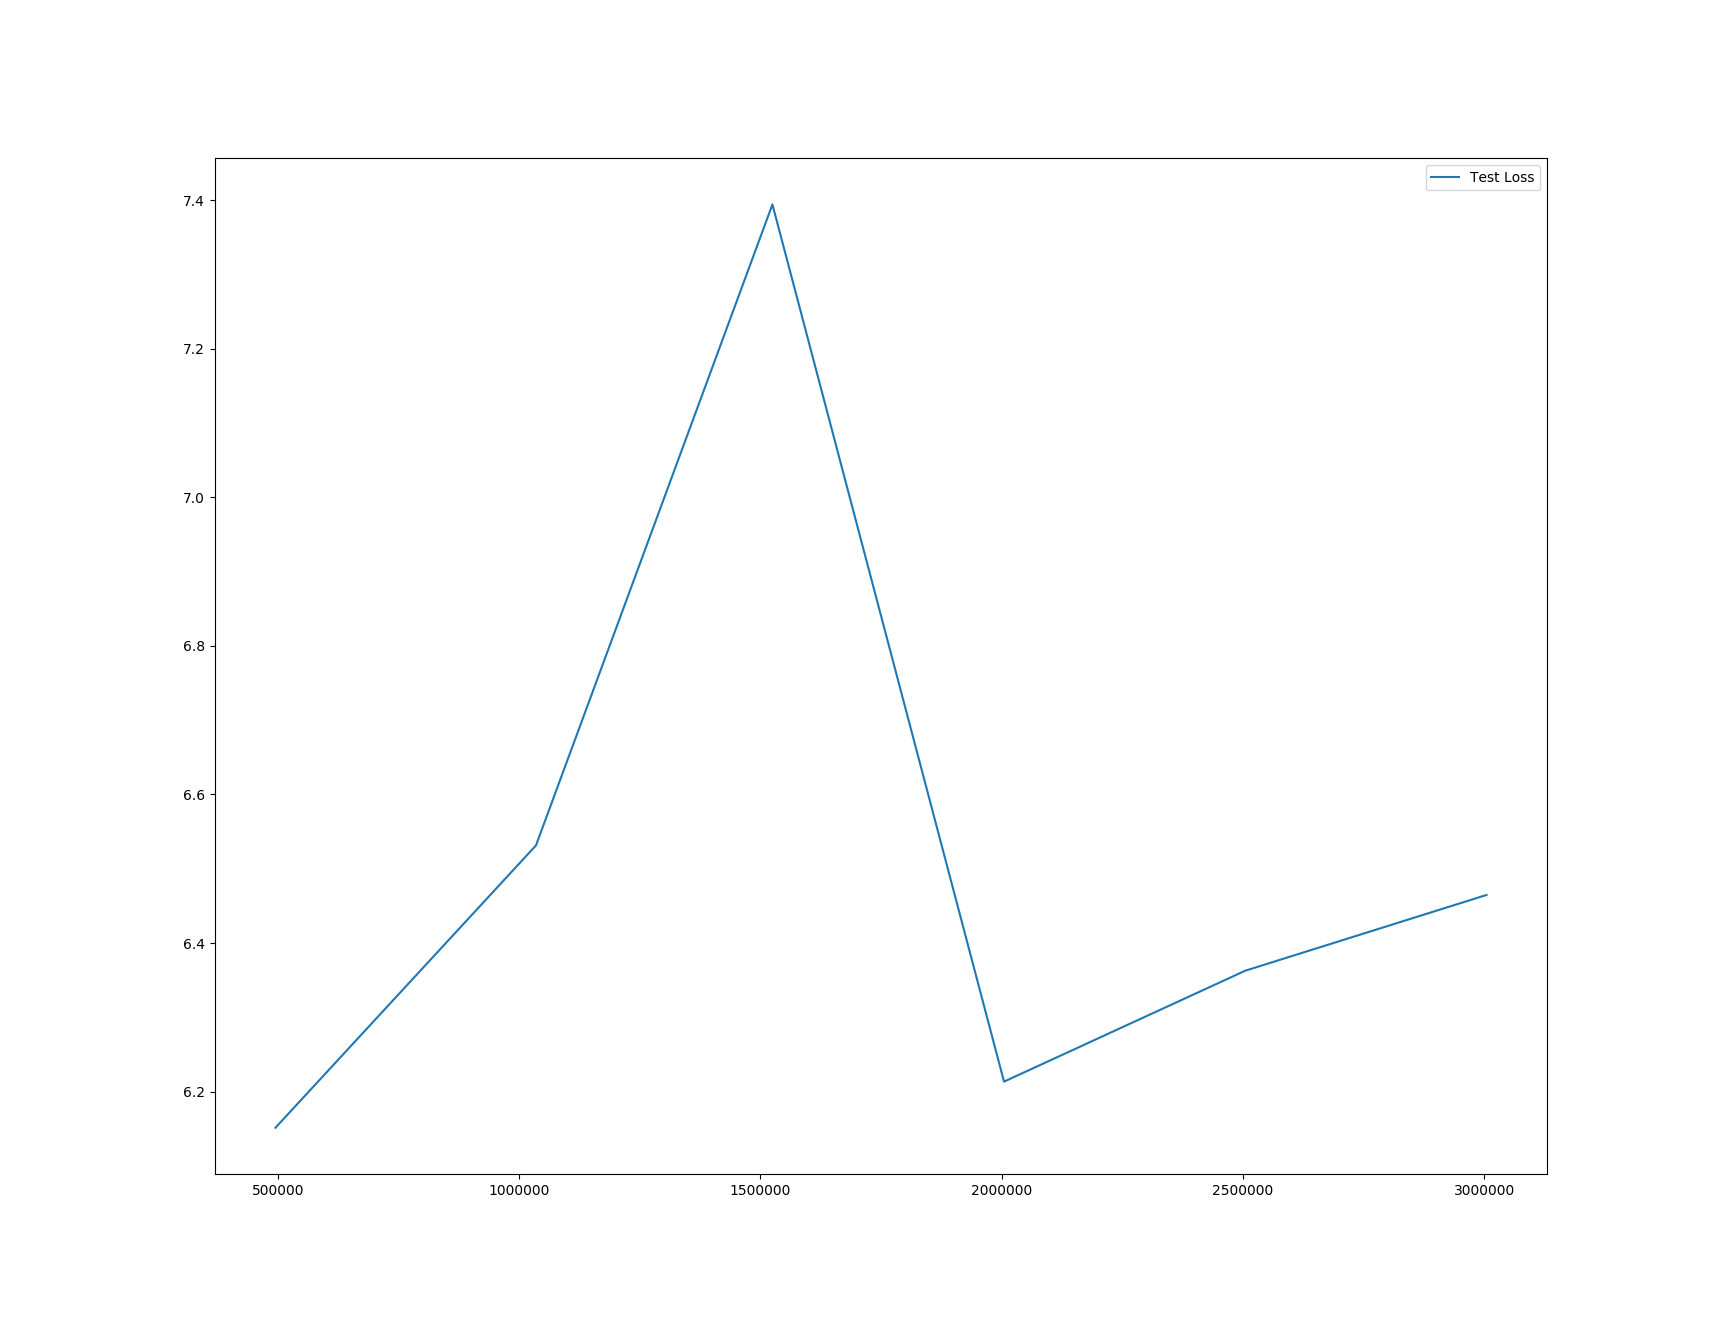
\includegraphics[width=\linewidth]{img/plots/opensubtitles_not_reversed/test_metrics_loss.png}
	\centering
	\small
	\text{Only the loss.}
	\endminipage\hfill
	\caption{The loss and perplexity by running the six different snapshots against the test dataset using the OpenSubtitles model.}
	\label{result:test_performance:opensubtitles}
\end{figure}

\begin{figure}[H]
	\minipage{0.5\textwidth}
	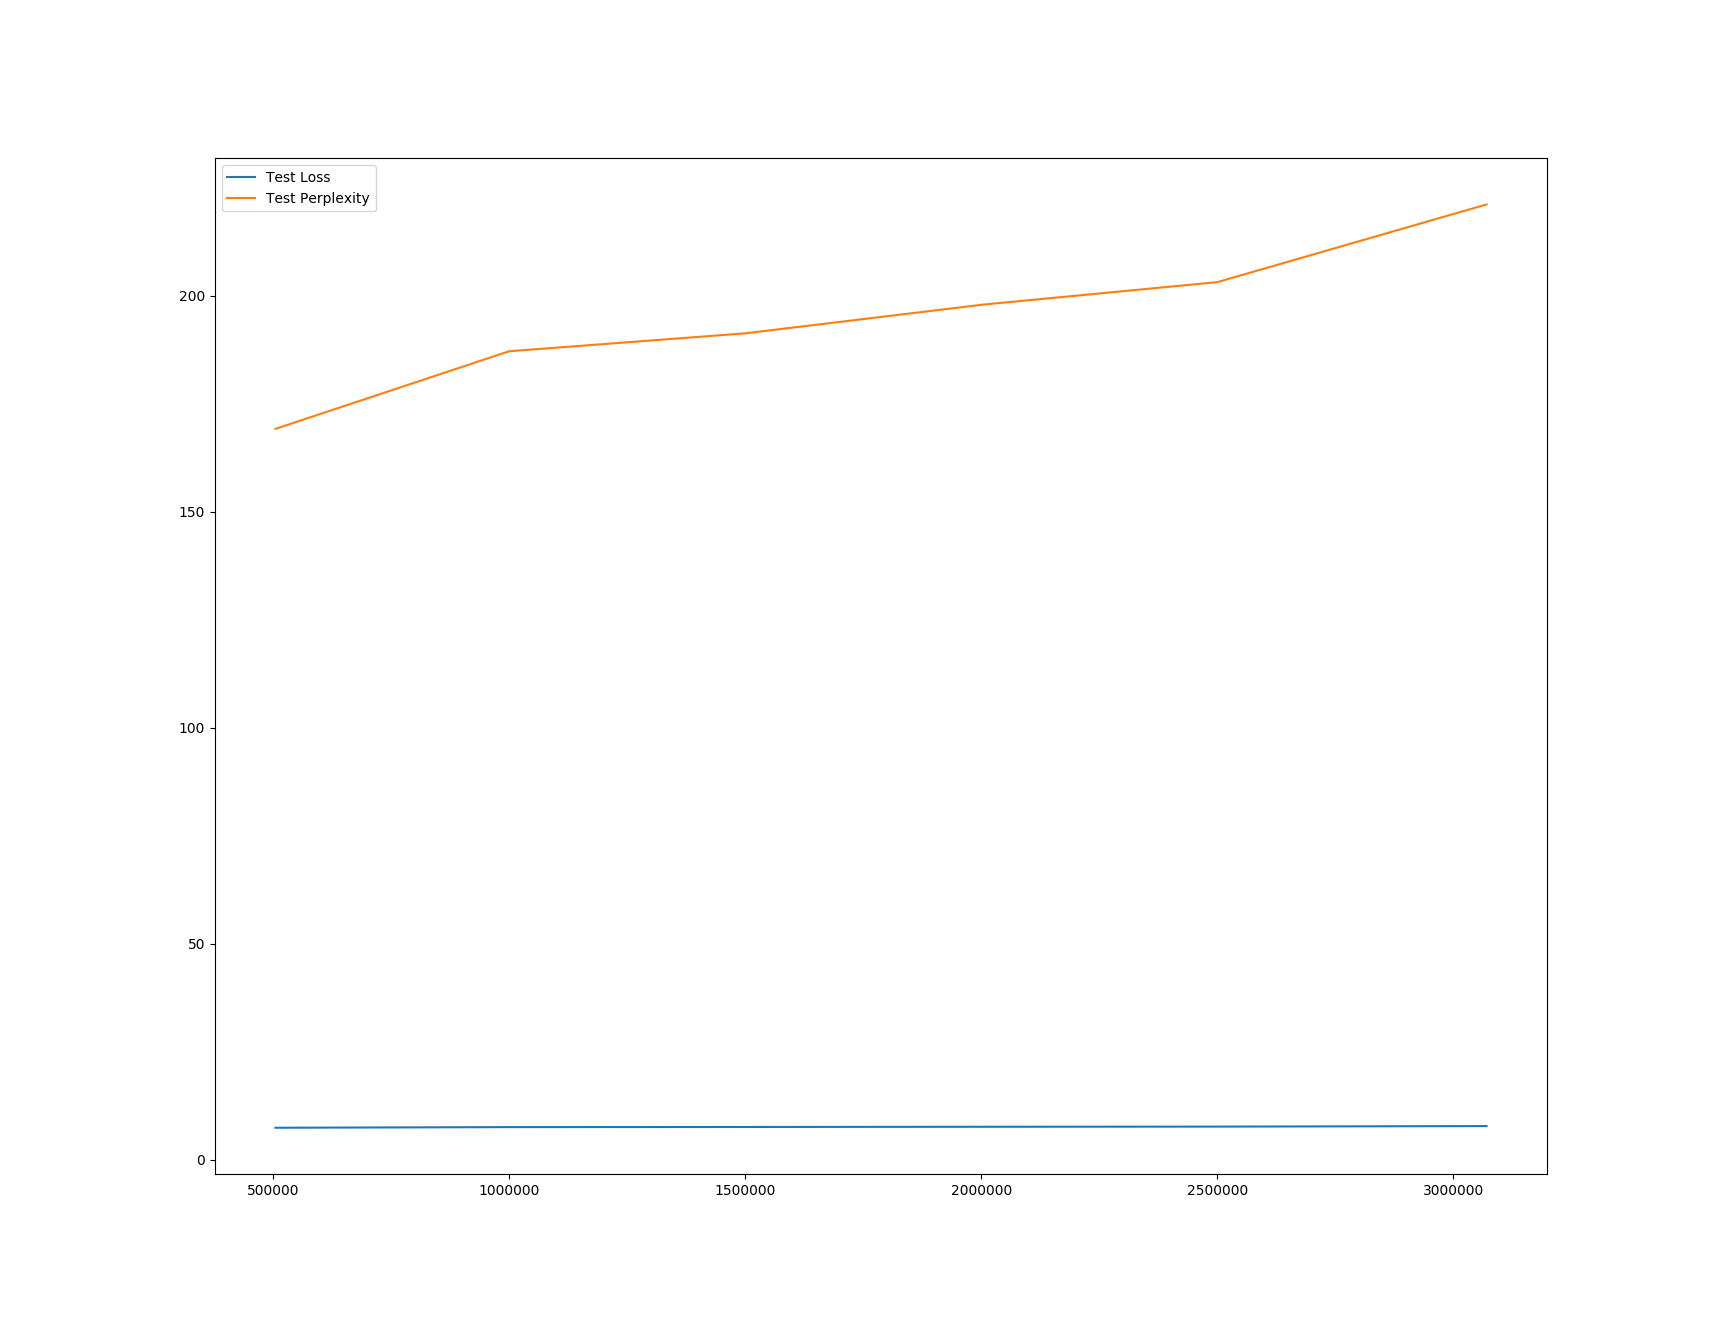
\includegraphics[width=\linewidth]{img/plots/reddit/test_metrics_both.png}
	\centering
	\small
	\text{The loss and perplexity.}
	\endminipage\hfill
	\minipage{0.5\textwidth}
	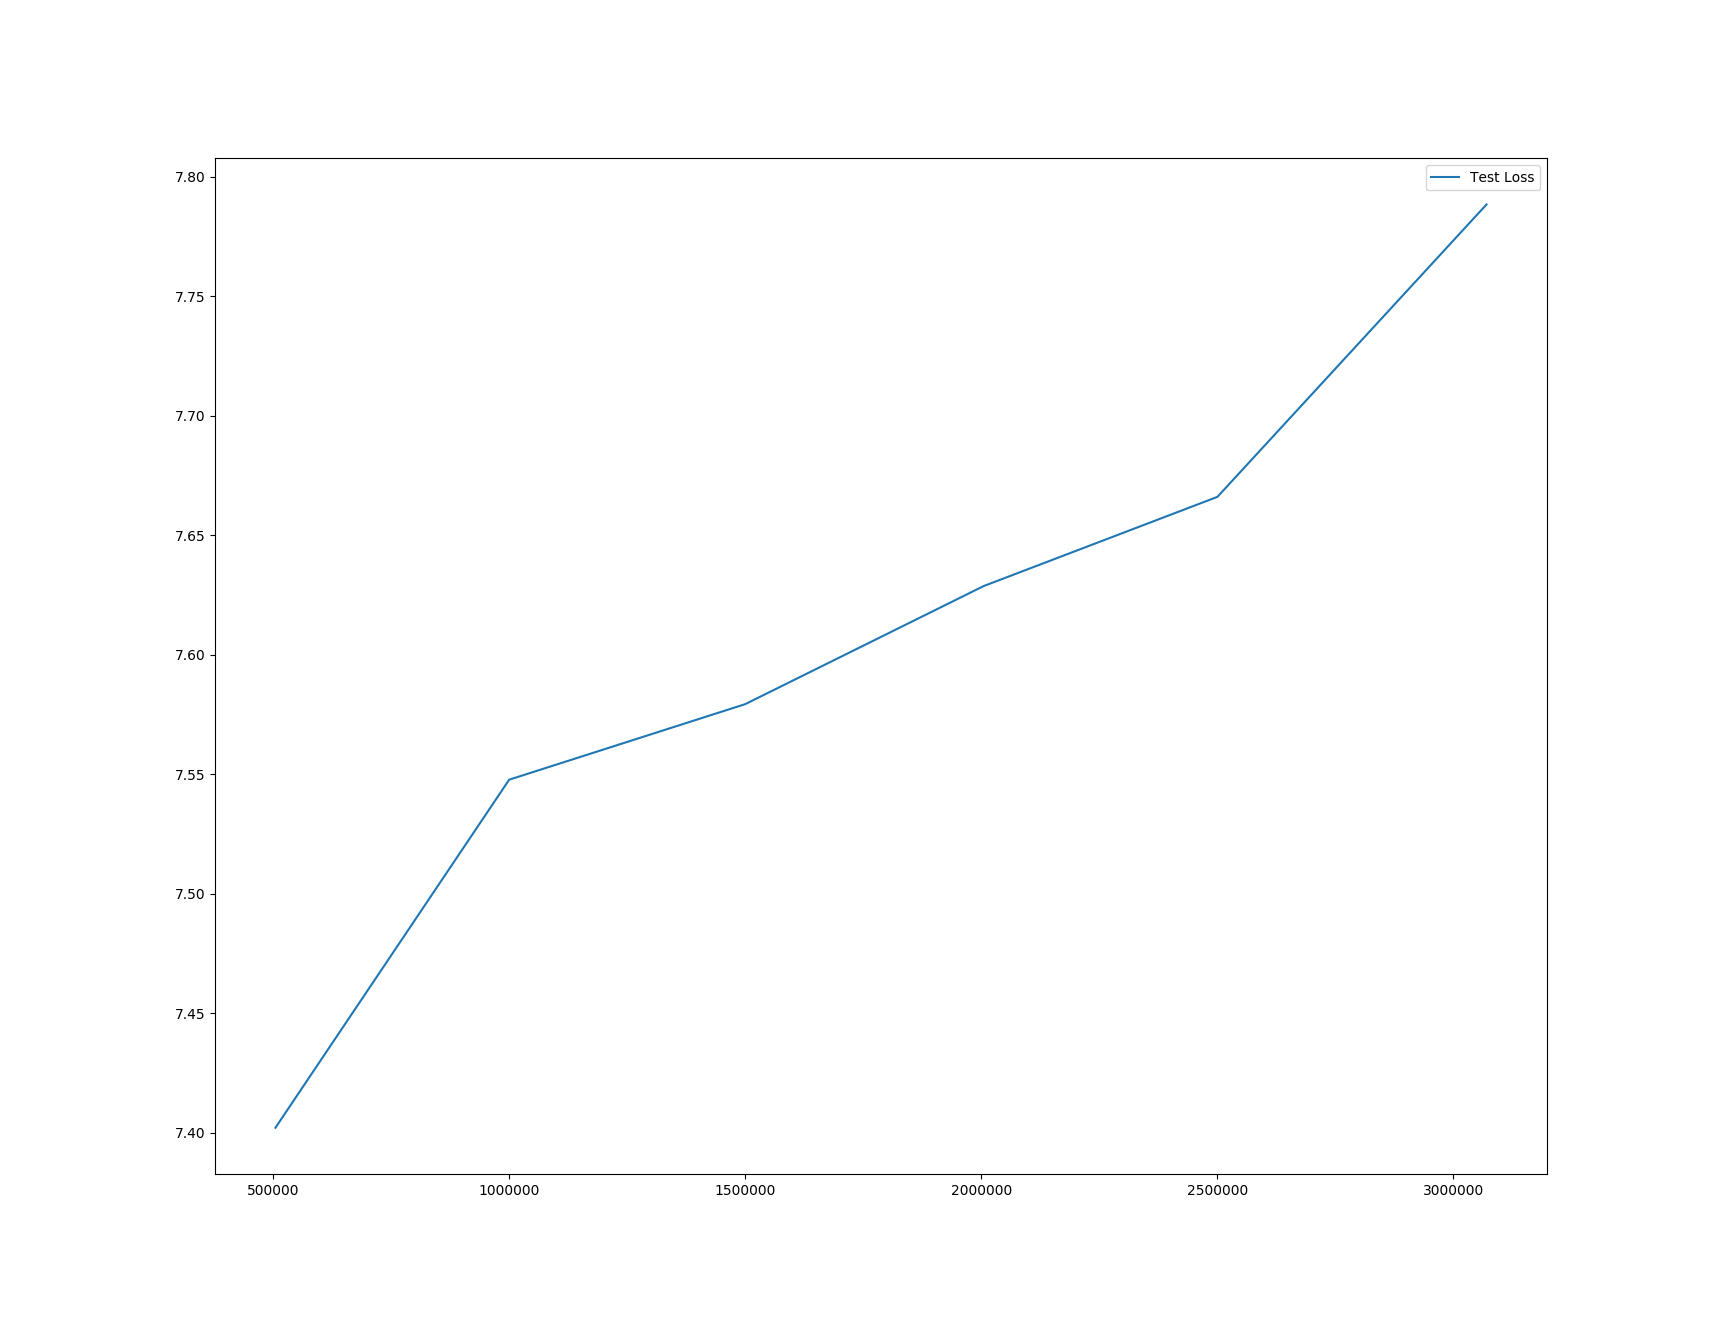
\includegraphics[width=\linewidth]{img/plots/reddit/test_metrics_loss.png}
	\centering
	\small
	\text{Only the loss.}
	\endminipage\hfill
	\caption{The loss and perplexity by running the six different snapshots against the test dataset using the Reddit model.}
	\label{result:test_performance:reddit}
\end{figure}

\section{Generated outputs over time}
\blindtext

\section{Comparison with CleverBot and ``Neural Conversational Model''}
\blindtext

\section{N-Gram Analysis}

\paragraph{OpenSubtitles} \blindtext
\begin{figure}[H]
	\minipage{0.5\textwidth}
	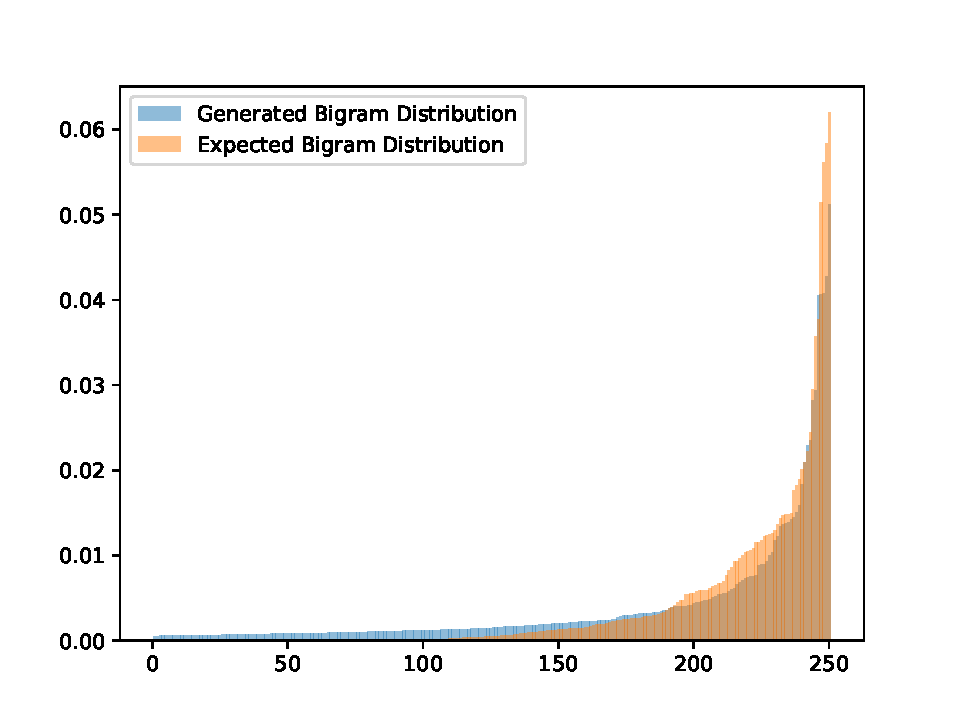
\includegraphics[width=\linewidth]{img/plots/opensubtitles_not_reversed/bigram_distribution_comparison_step_500000.pdf}
	\centering
	\small
	\text{Distribution at training step 500'000.}
	\endminipage\hfill
	\minipage{0.5\textwidth}
	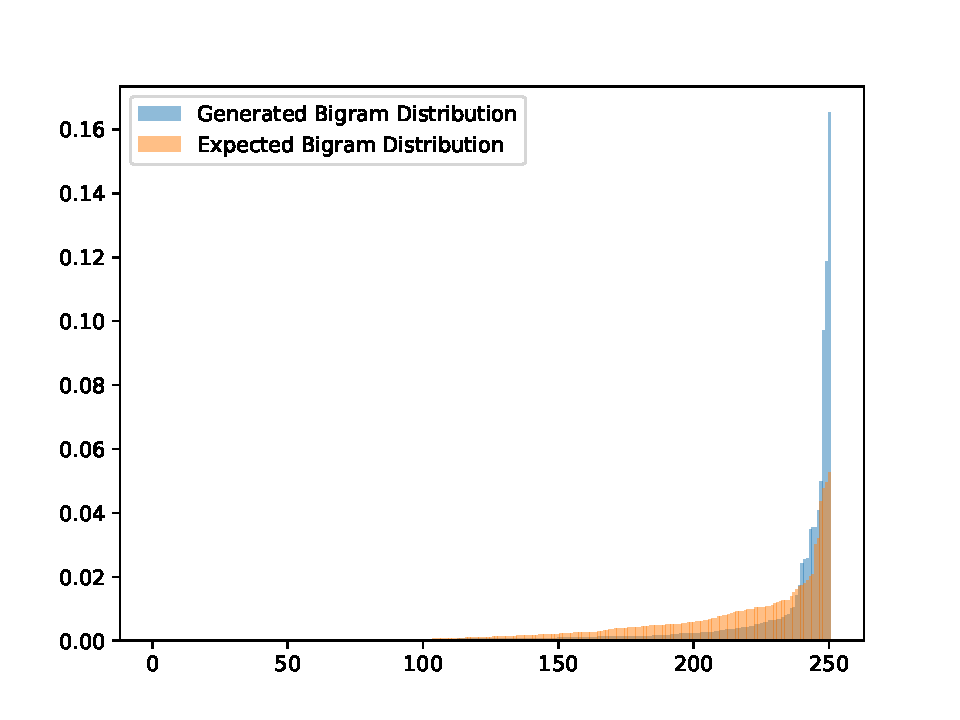
\includegraphics[width=\linewidth]{img/plots/opensubtitles_not_reversed/bigram_distribution_comparison_step_1000000.pdf}
	\centering
	\small
	\text{Distribution at training step 1'000'000.}
	\endminipage\hfill
	\minipage{0.5\textwidth}
	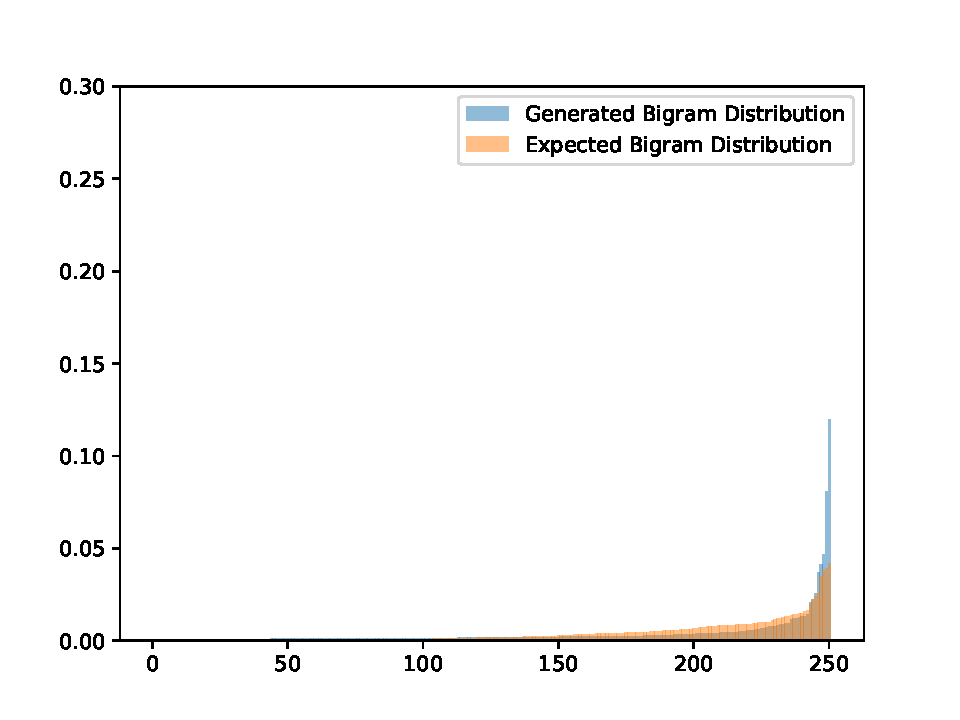
\includegraphics[width=\linewidth]{img/plots/opensubtitles_not_reversed/bigram_distribution_comparison_step_1500000.pdf}
	\centering
	\small
	\text{Distribution at training step 1'500'000.}
	\endminipage\hfill
	\minipage{0.5\textwidth}
	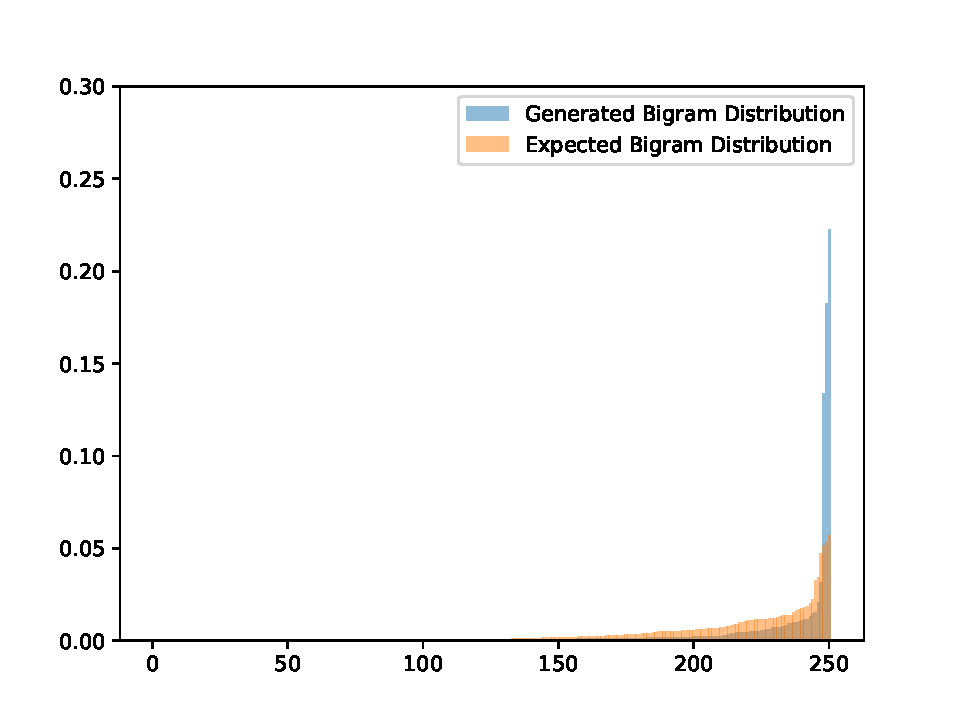
\includegraphics[width=\linewidth]{img/plots/opensubtitles_not_reversed/bigram_distribution_comparison_step_2000000.pdf}
	\centering
	\small
	\text{Distribution at training step 2'000'000.}
	\endminipage\hfill
	\minipage{0.5\textwidth}
	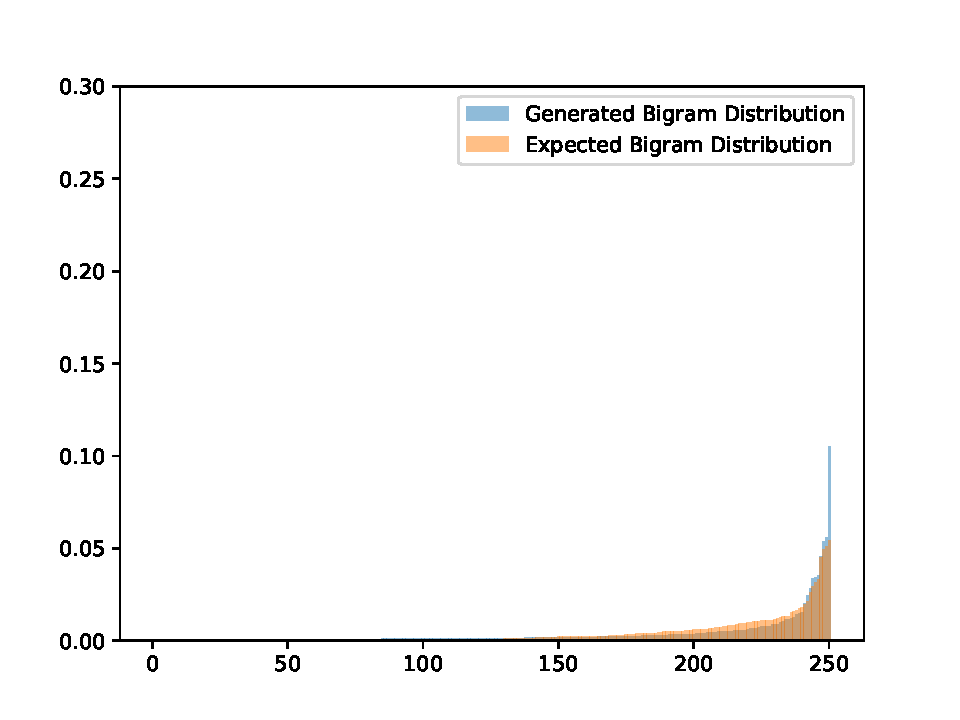
\includegraphics[width=\linewidth]{img/plots/opensubtitles_not_reversed/bigram_distribution_comparison_step_2500000.pdf}
	\centering
	\small
	\text{Distribution at training step 2'500'000.}
	\endminipage\hfill
	\minipage{0.5\textwidth}
	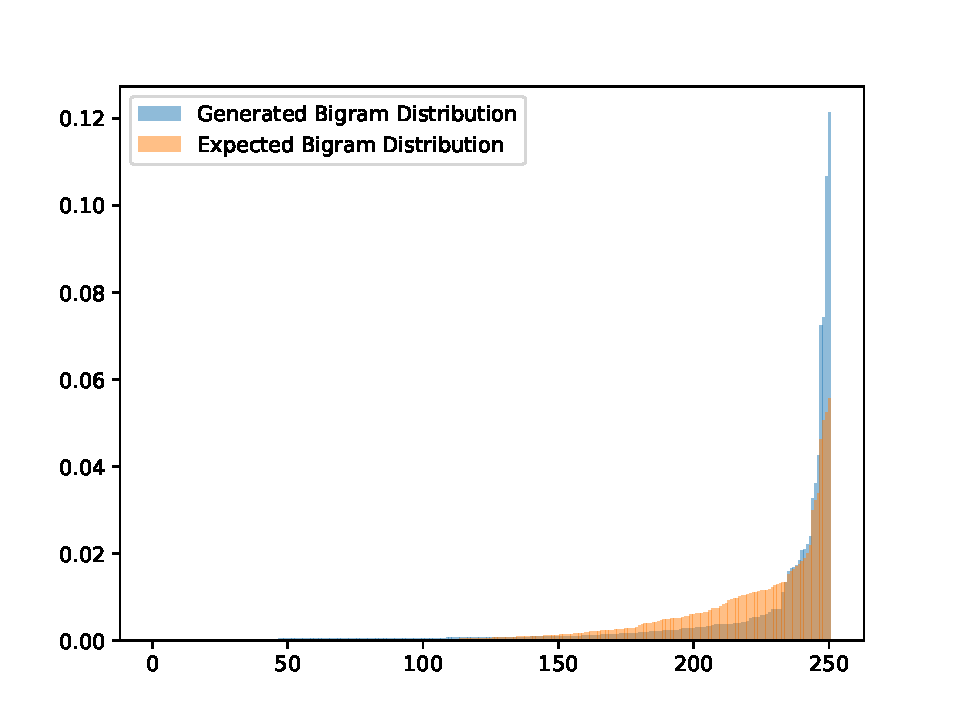
\includegraphics[width=\linewidth]{img/plots/opensubtitles_not_reversed/bigram_distribution_comparison_step_3000000.pdf}
	\centering
	\small
	\text{Distribution at training step 3'000'000.}
	\endminipage\hfill
	\caption{Distributions of the top 100 bigrams in the generated answers when using the test set over multiple time steps of the training.}
	\label{results:ngram:distributions:opensubtitles}
\end{figure}

\paragraph{Reddit} \blindtext
\begin{figure}[H]
	\minipage{0.5\textwidth}
	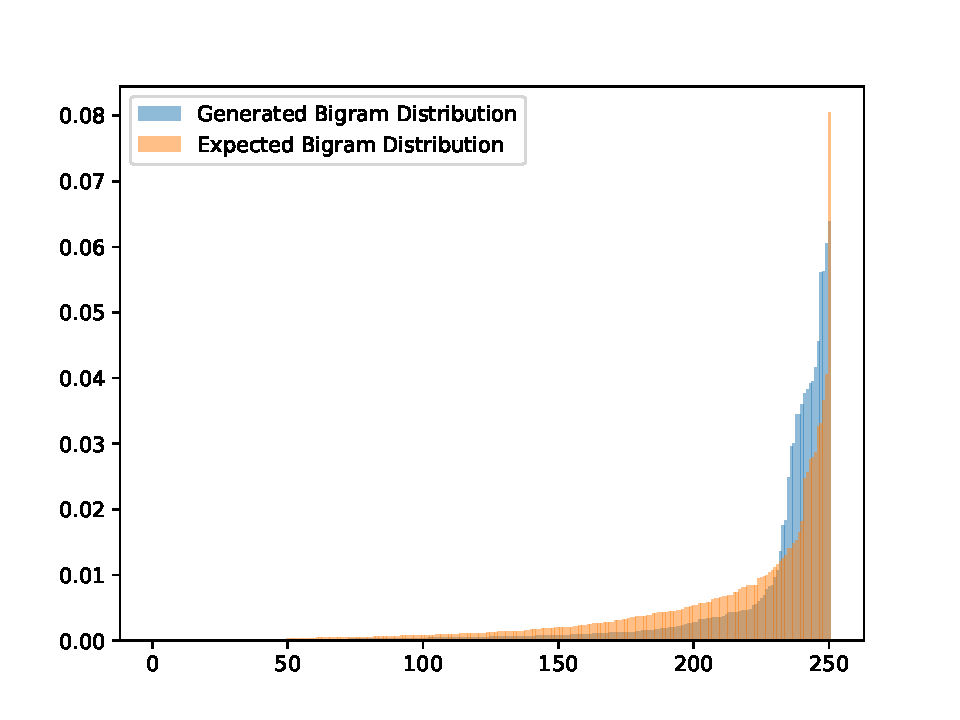
\includegraphics[width=\linewidth]{img/plots/reddit/bigram_distribution_comparison_step_500000.pdf}
	\centering
	\small
	\text{Distribution at training step 500'000.}
	\endminipage\hfill
	\minipage{0.5\textwidth}
	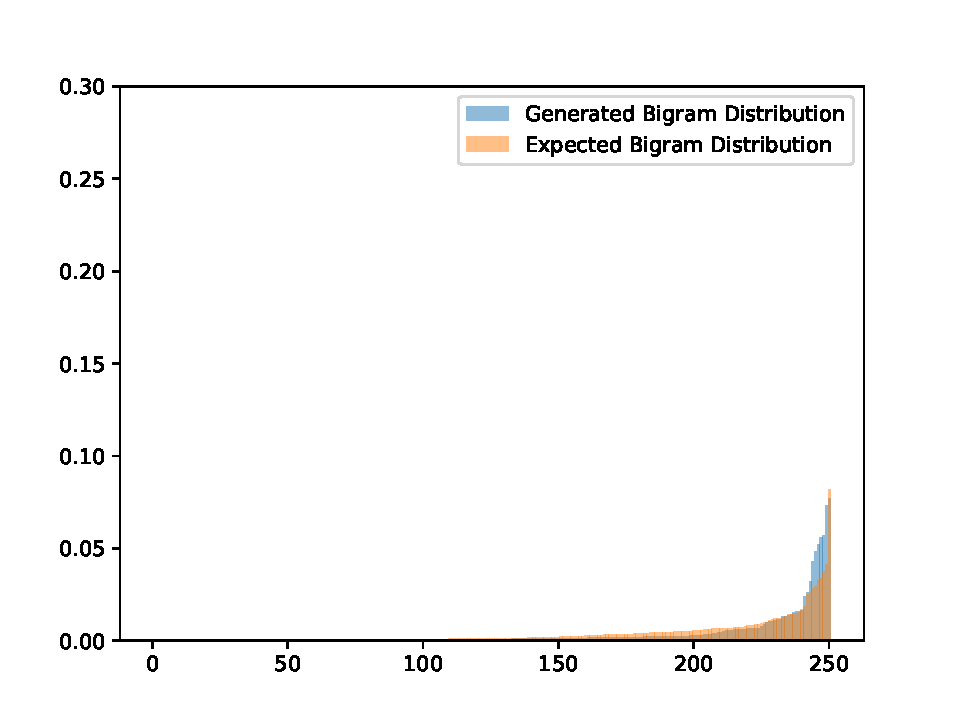
\includegraphics[width=\linewidth]{img/plots/reddit/bigram_distribution_comparison_step_1000000.pdf}
	\centering
	\small
	\text{Distribution at training step 1'000'000.}
	\endminipage\hfill
	\minipage{0.5\textwidth}
	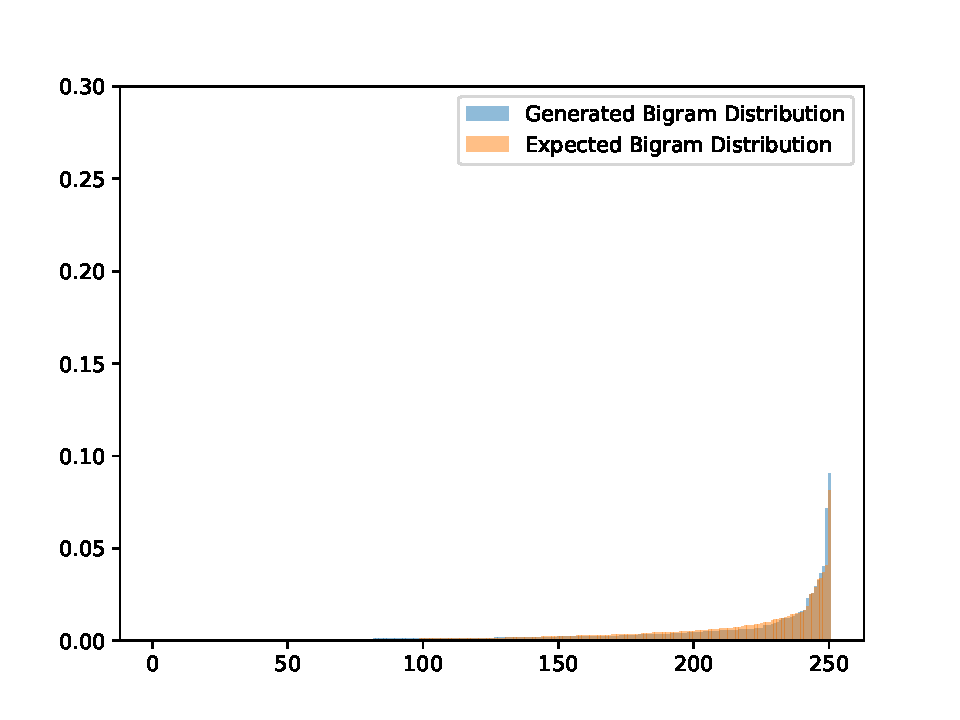
\includegraphics[width=\linewidth]{img/plots/reddit/bigram_distribution_comparison_step_1500000.pdf}
	\centering
	\small
	\text{Distribution at training step 1'500'000.}
	\endminipage\hfill
	\minipage{0.5\textwidth}
	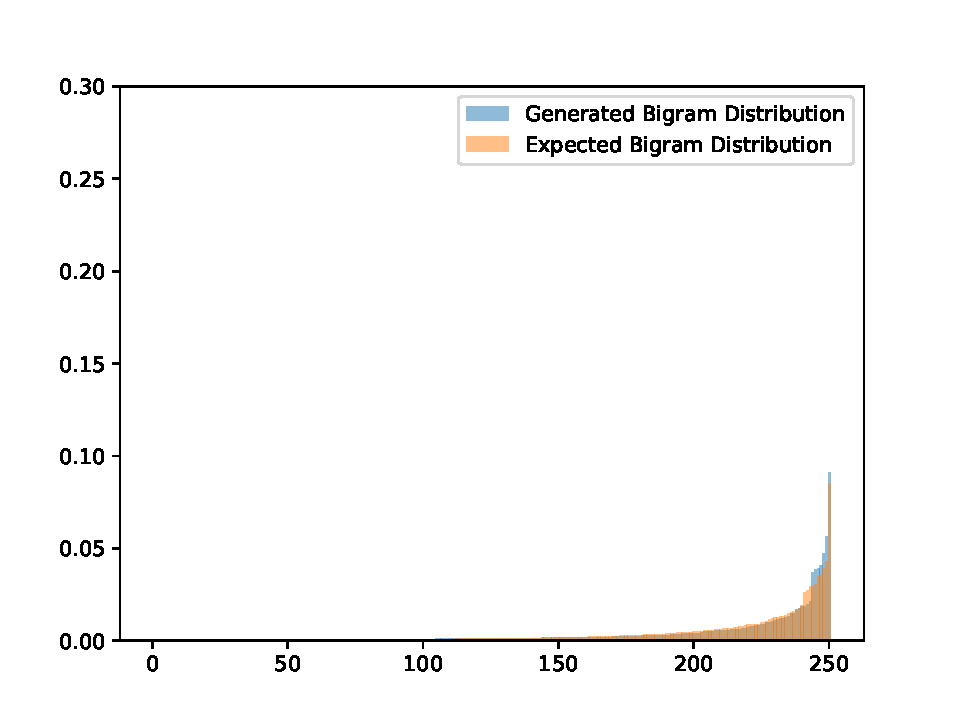
\includegraphics[width=\linewidth]{img/plots/reddit/bigram_distribution_comparison_step_2000000.pdf}
	\centering
	\small
	\text{Distribution at training step 2'000'000.}
	\endminipage\hfill
	\minipage{0.5\textwidth}
	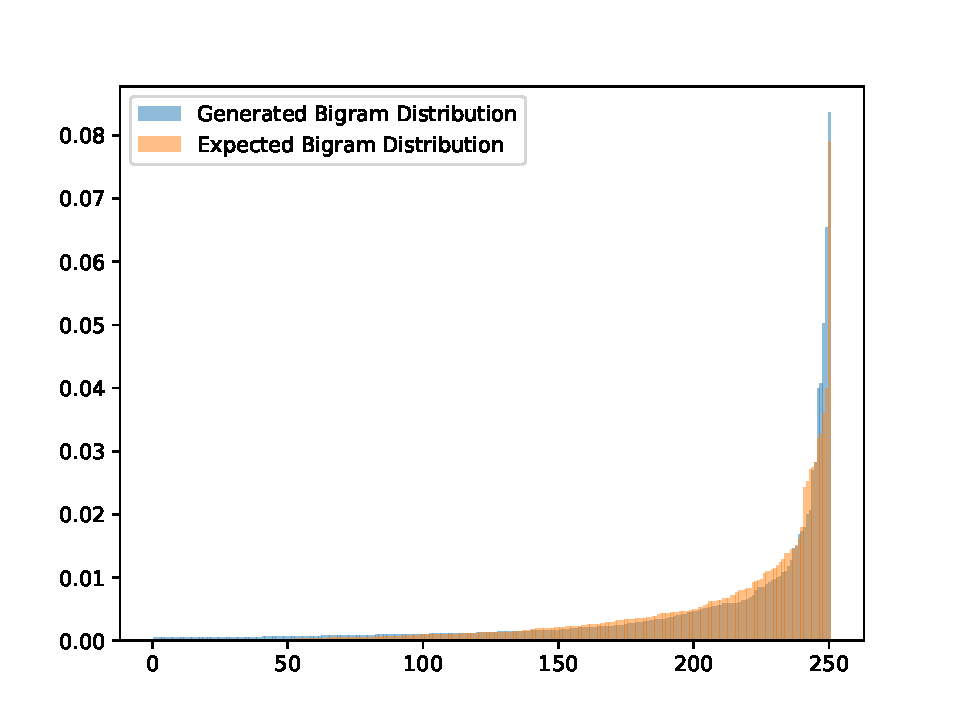
\includegraphics[width=\linewidth]{img/plots/reddit/bigram_distribution_comparison_step_2500000.pdf}
	\centering
	\small
	\text{Distribution at training step 2'500'000.}
	\endminipage\hfill
	\minipage{0.5\textwidth}
	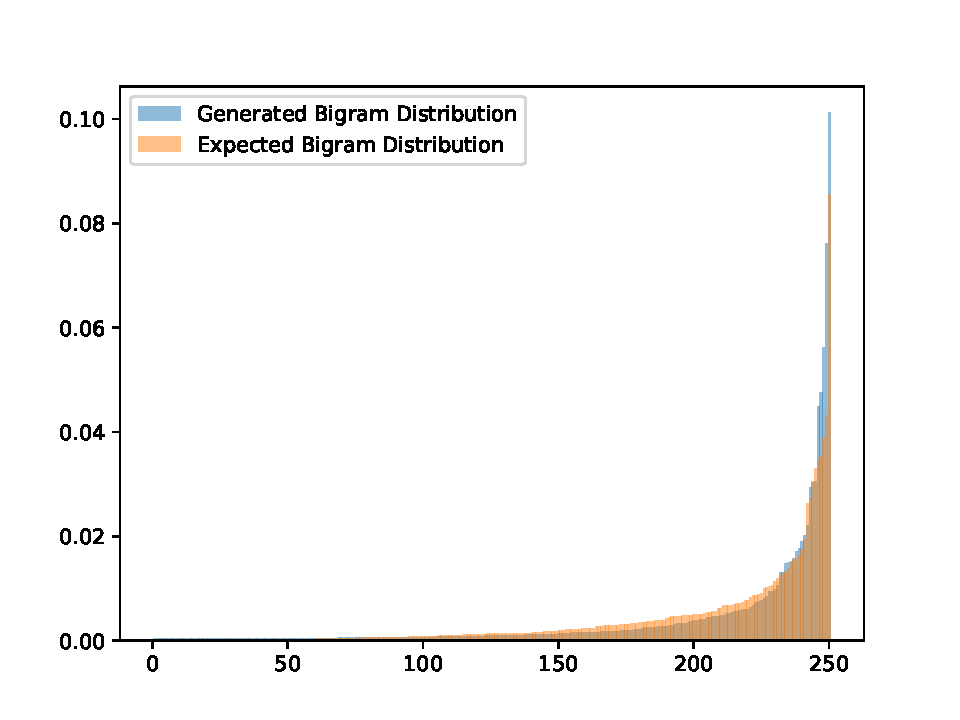
\includegraphics[width=\linewidth]{img/plots/reddit/bigram_distribution_comparison_step_3000000.pdf}
	\centering
	\small
	\text{Distribution at training step 3'000'000.}
	\endminipage\hfill
	\caption{Distributions of the top 100 bigrams in the generated answers when using the test set over multiple time steps of the training.}
	\label{results:ngram:distributions:opensubtitles}
\end{figure}

\section{Sent2Vec Analysis}

\begin{figure}[H]
	\minipage{0.5\textwidth}
	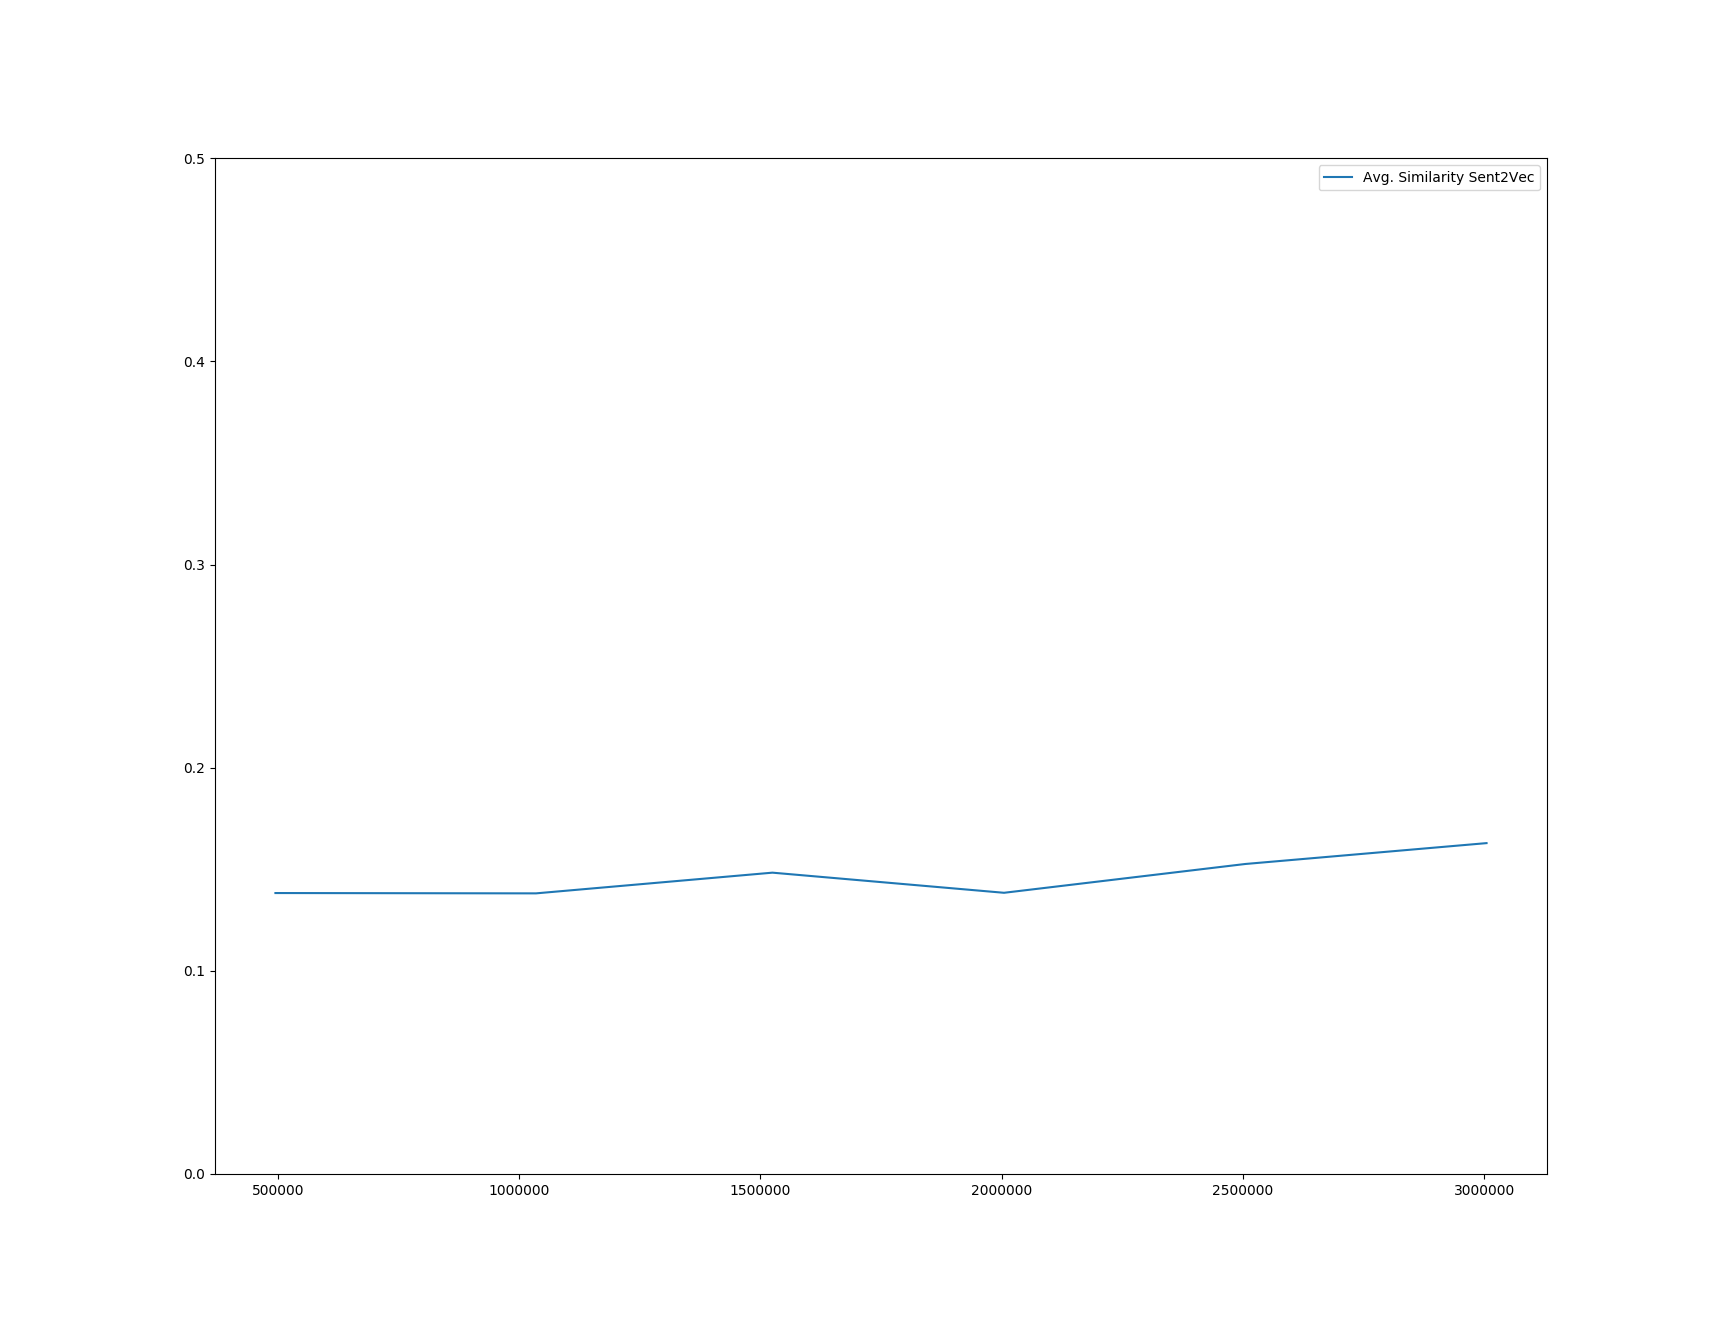
\includegraphics[width=\linewidth]{img/plots/opensubtitles_not_reversed/s2v_wiki_cosine_similarity.png}
	\centering
	\small
	\text{Evaluation with the wiki model.}
	\endminipage\hfill
	\minipage{0.5\textwidth}
	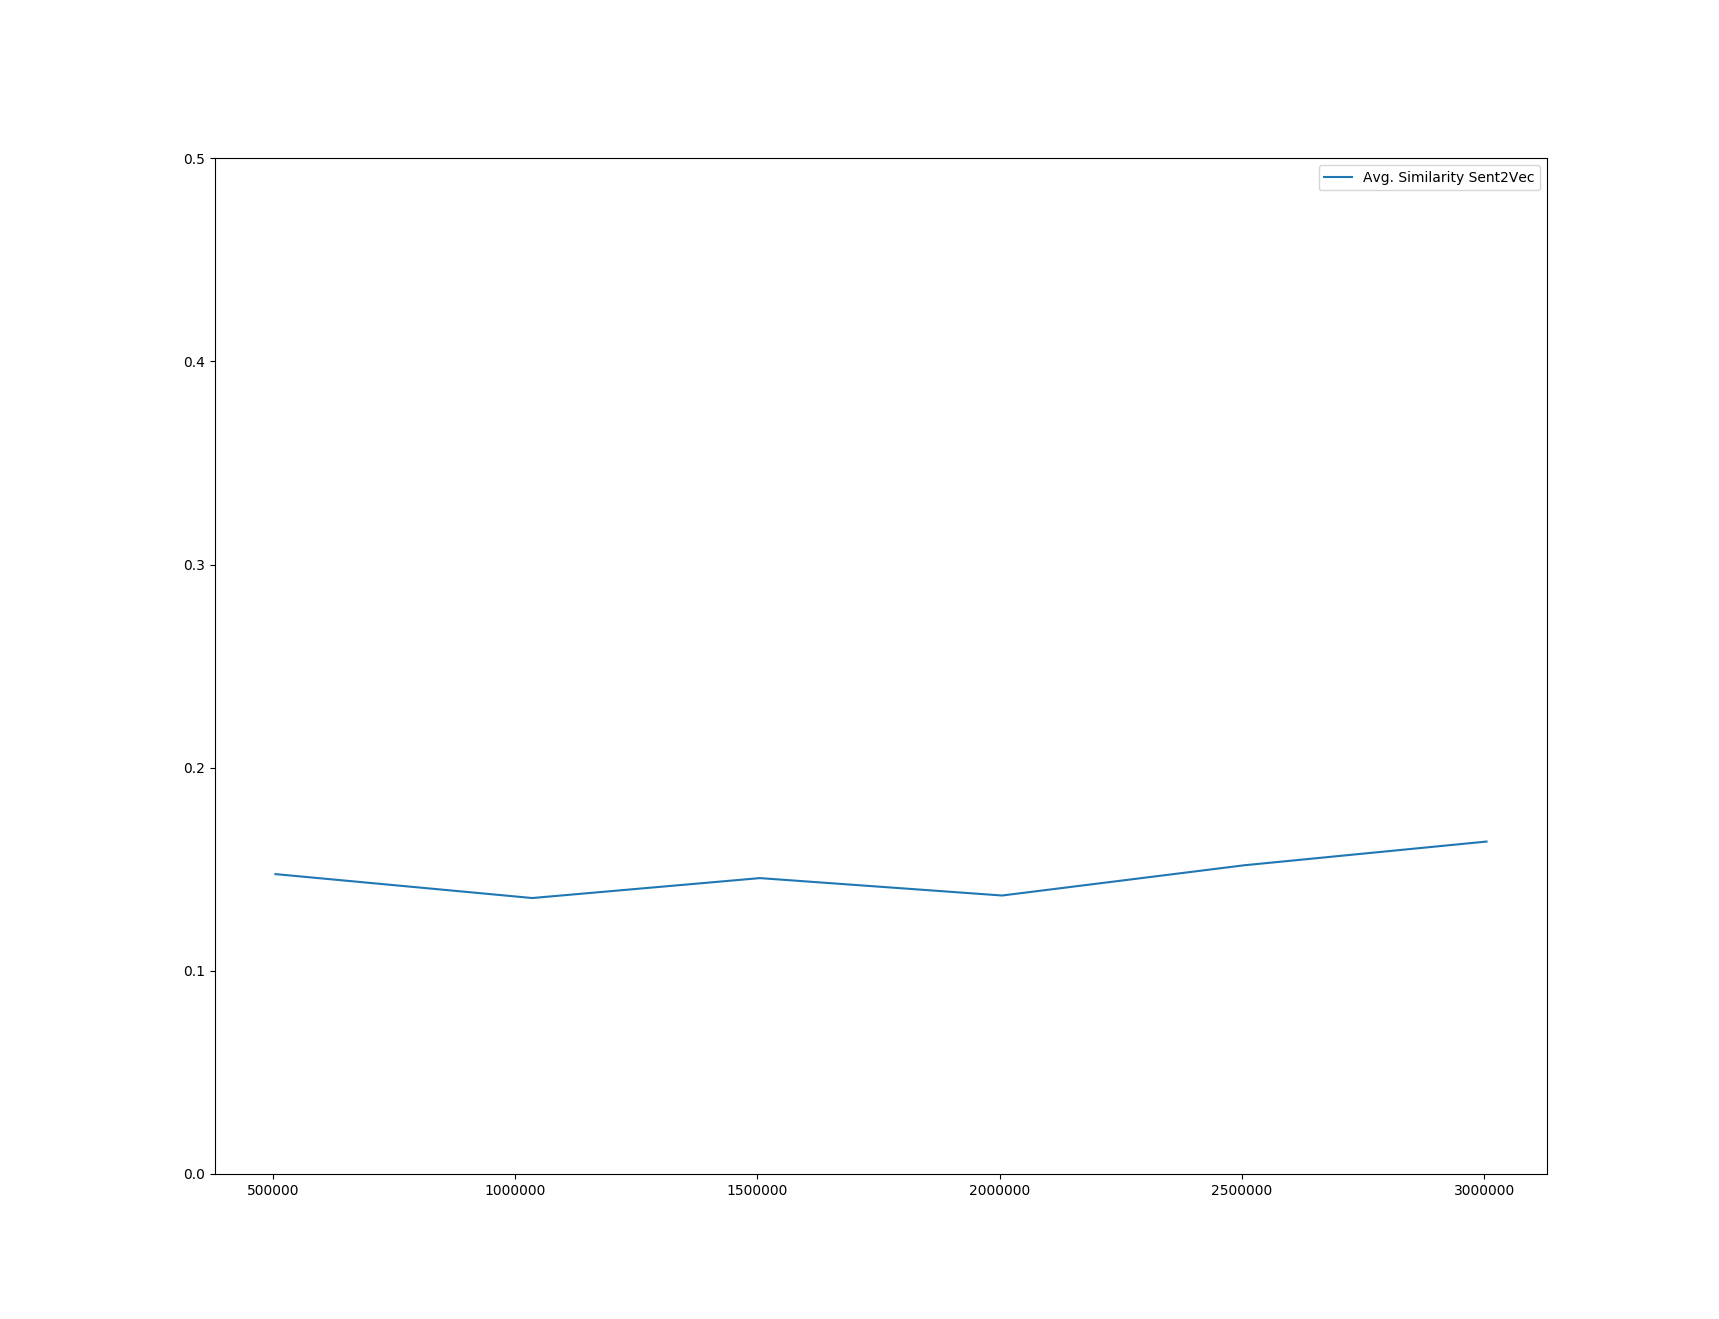
\includegraphics[width=\linewidth]{img/plots/opensubtitles_not_reversed/s2v_twitter_cosine_similarity.png}
	\centering
	\small
	\text{Evaluation with the twitter model.}
	\endminipage\hfill
	\caption{Results of the evaluation with Sent2Vec on the outputs of the OpenSubtitles models using the pretrained models found on the Sent2Vec GitHub page.}
	\label{results:sent2vec:opensubtitles:results}
\end{figure}

\begin{figure}[H]
	\minipage{0.5\textwidth}
	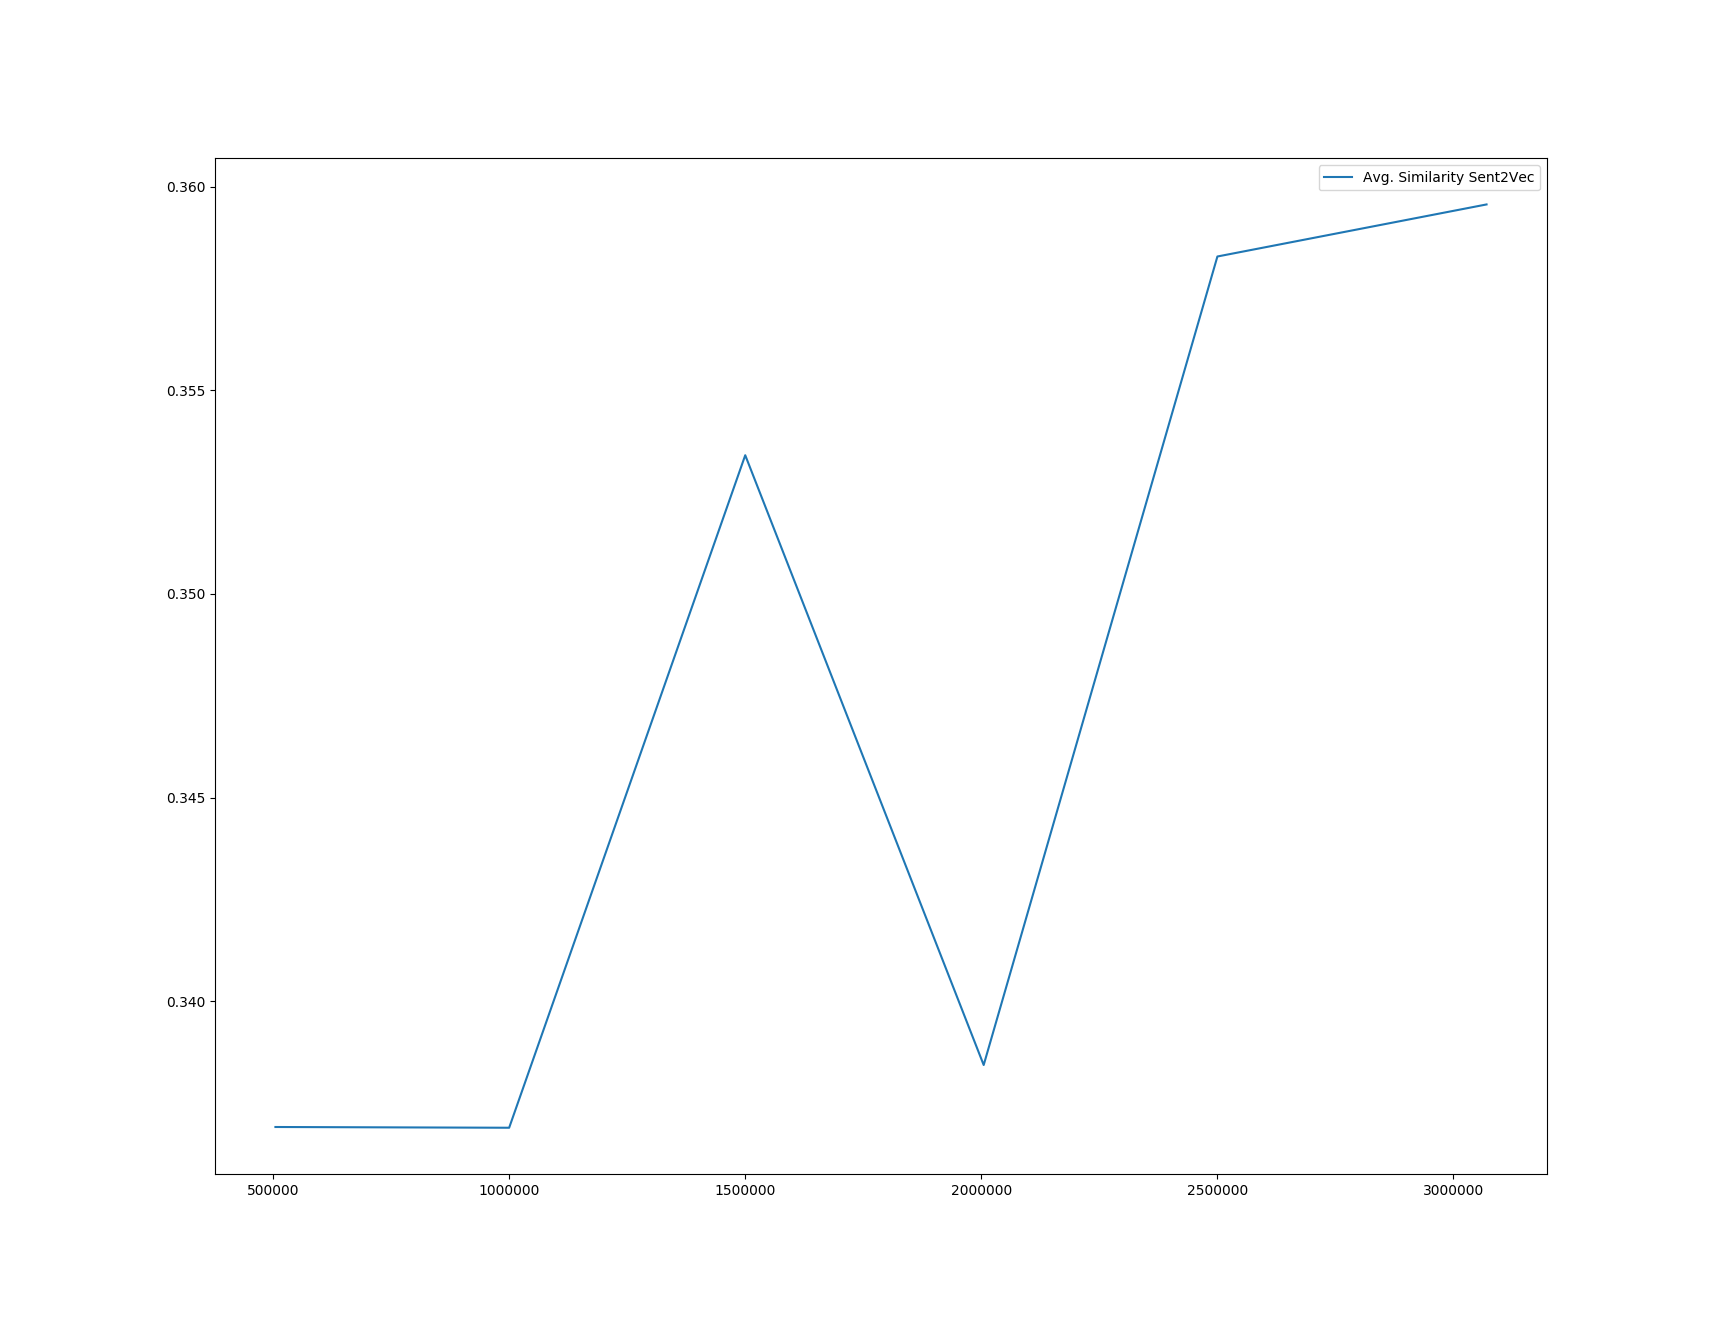
\includegraphics[width=\linewidth]{img/plots/reddit/s2v_wiki_cosine_similarity.png}
	\centering
	\small
	\text{Evaluation with the wiki model.}
	\endminipage\hfill
	\minipage{0.5\textwidth}
	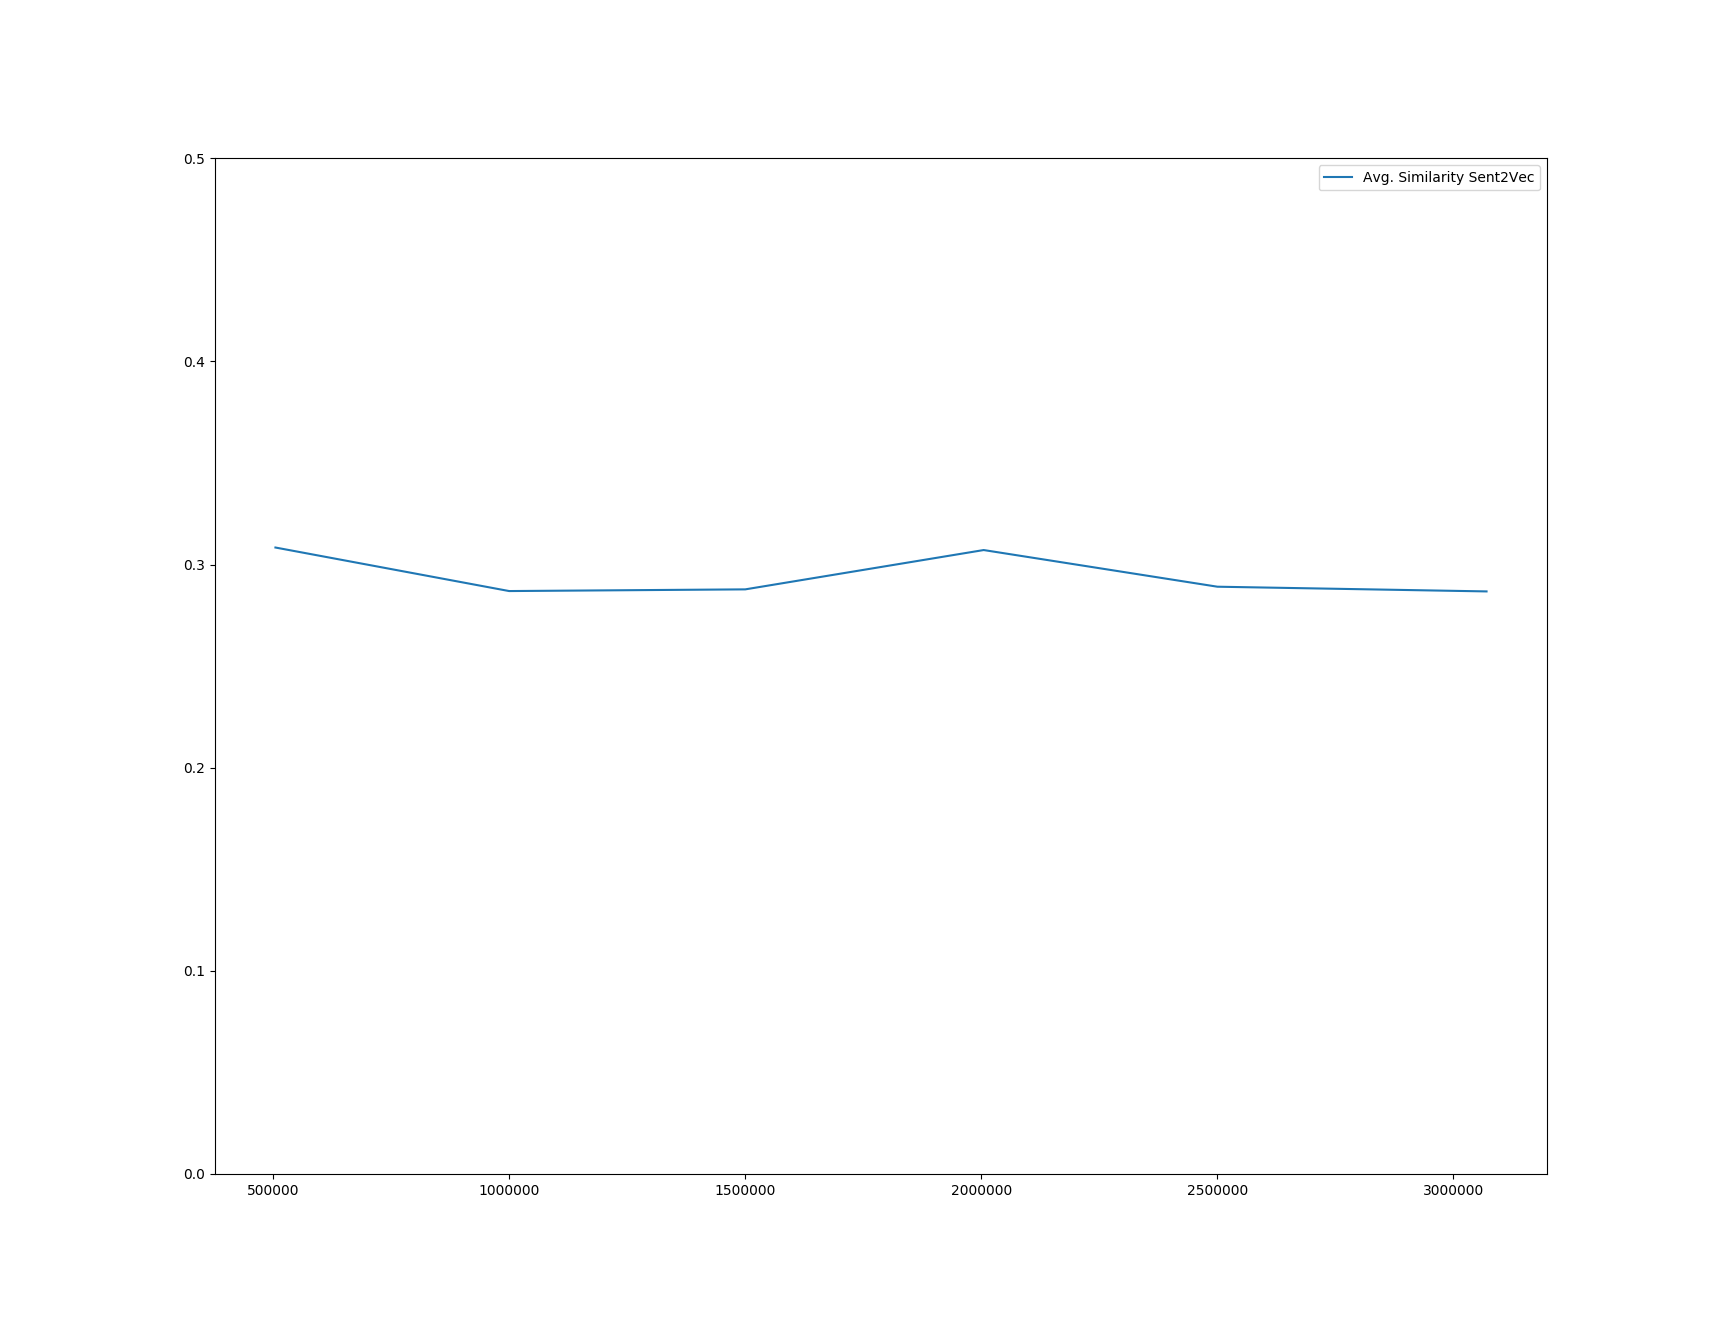
\includegraphics[width=\linewidth]{img/plots/reddit/s2v_twitter_cosine_similarity.png}
	\centering
	\small
	\text{Evaluation with the twitter model.}
	\endminipage\hfill
	\caption{Results of the evaluation with Sent2Vec on the outputs of the Reddit models using the pretrained models found on the Sent2Vec GitHub page.}
	\label{results:sent2vec:reddit:results}
\end{figure}
\footnotetext{https://github.com/epfml/sent2vec}

\section{Internal Embedding for Input Sequences}
\blindtext